\documentclass{article}
\usepackage[margin=0.5in]{geometry}
\usepackage{pdflscape}
\usepackage{amssymb}
\usepackage{xcolor}
\usepackage{tikz}
\usetikzlibrary{positioning, shapes.geometric}

% Define custom colors
\definecolor{darkblue}{RGB}{25,25,112}
\definecolor{lightblue}{RGB}{173,216,230}
\definecolor{darkred}{RGB}{139,0,0}
\definecolor{darkgreen}{RGB}{0,100,0}
\definecolor{purple}{RGB}{128,0,128}

\begin{document}
\thispagestyle{empty}
\begin{landscape}

\begin{center}
{\Huge\bfseries\color{darkblue} HUNT THE SITH}\\[0.5cm]
{\Large\itshape A Choose Your Own Adventure Decision Tree}
\end{center}

\vspace{1cm}

\resizebox{1.2\textwidth}{!}{
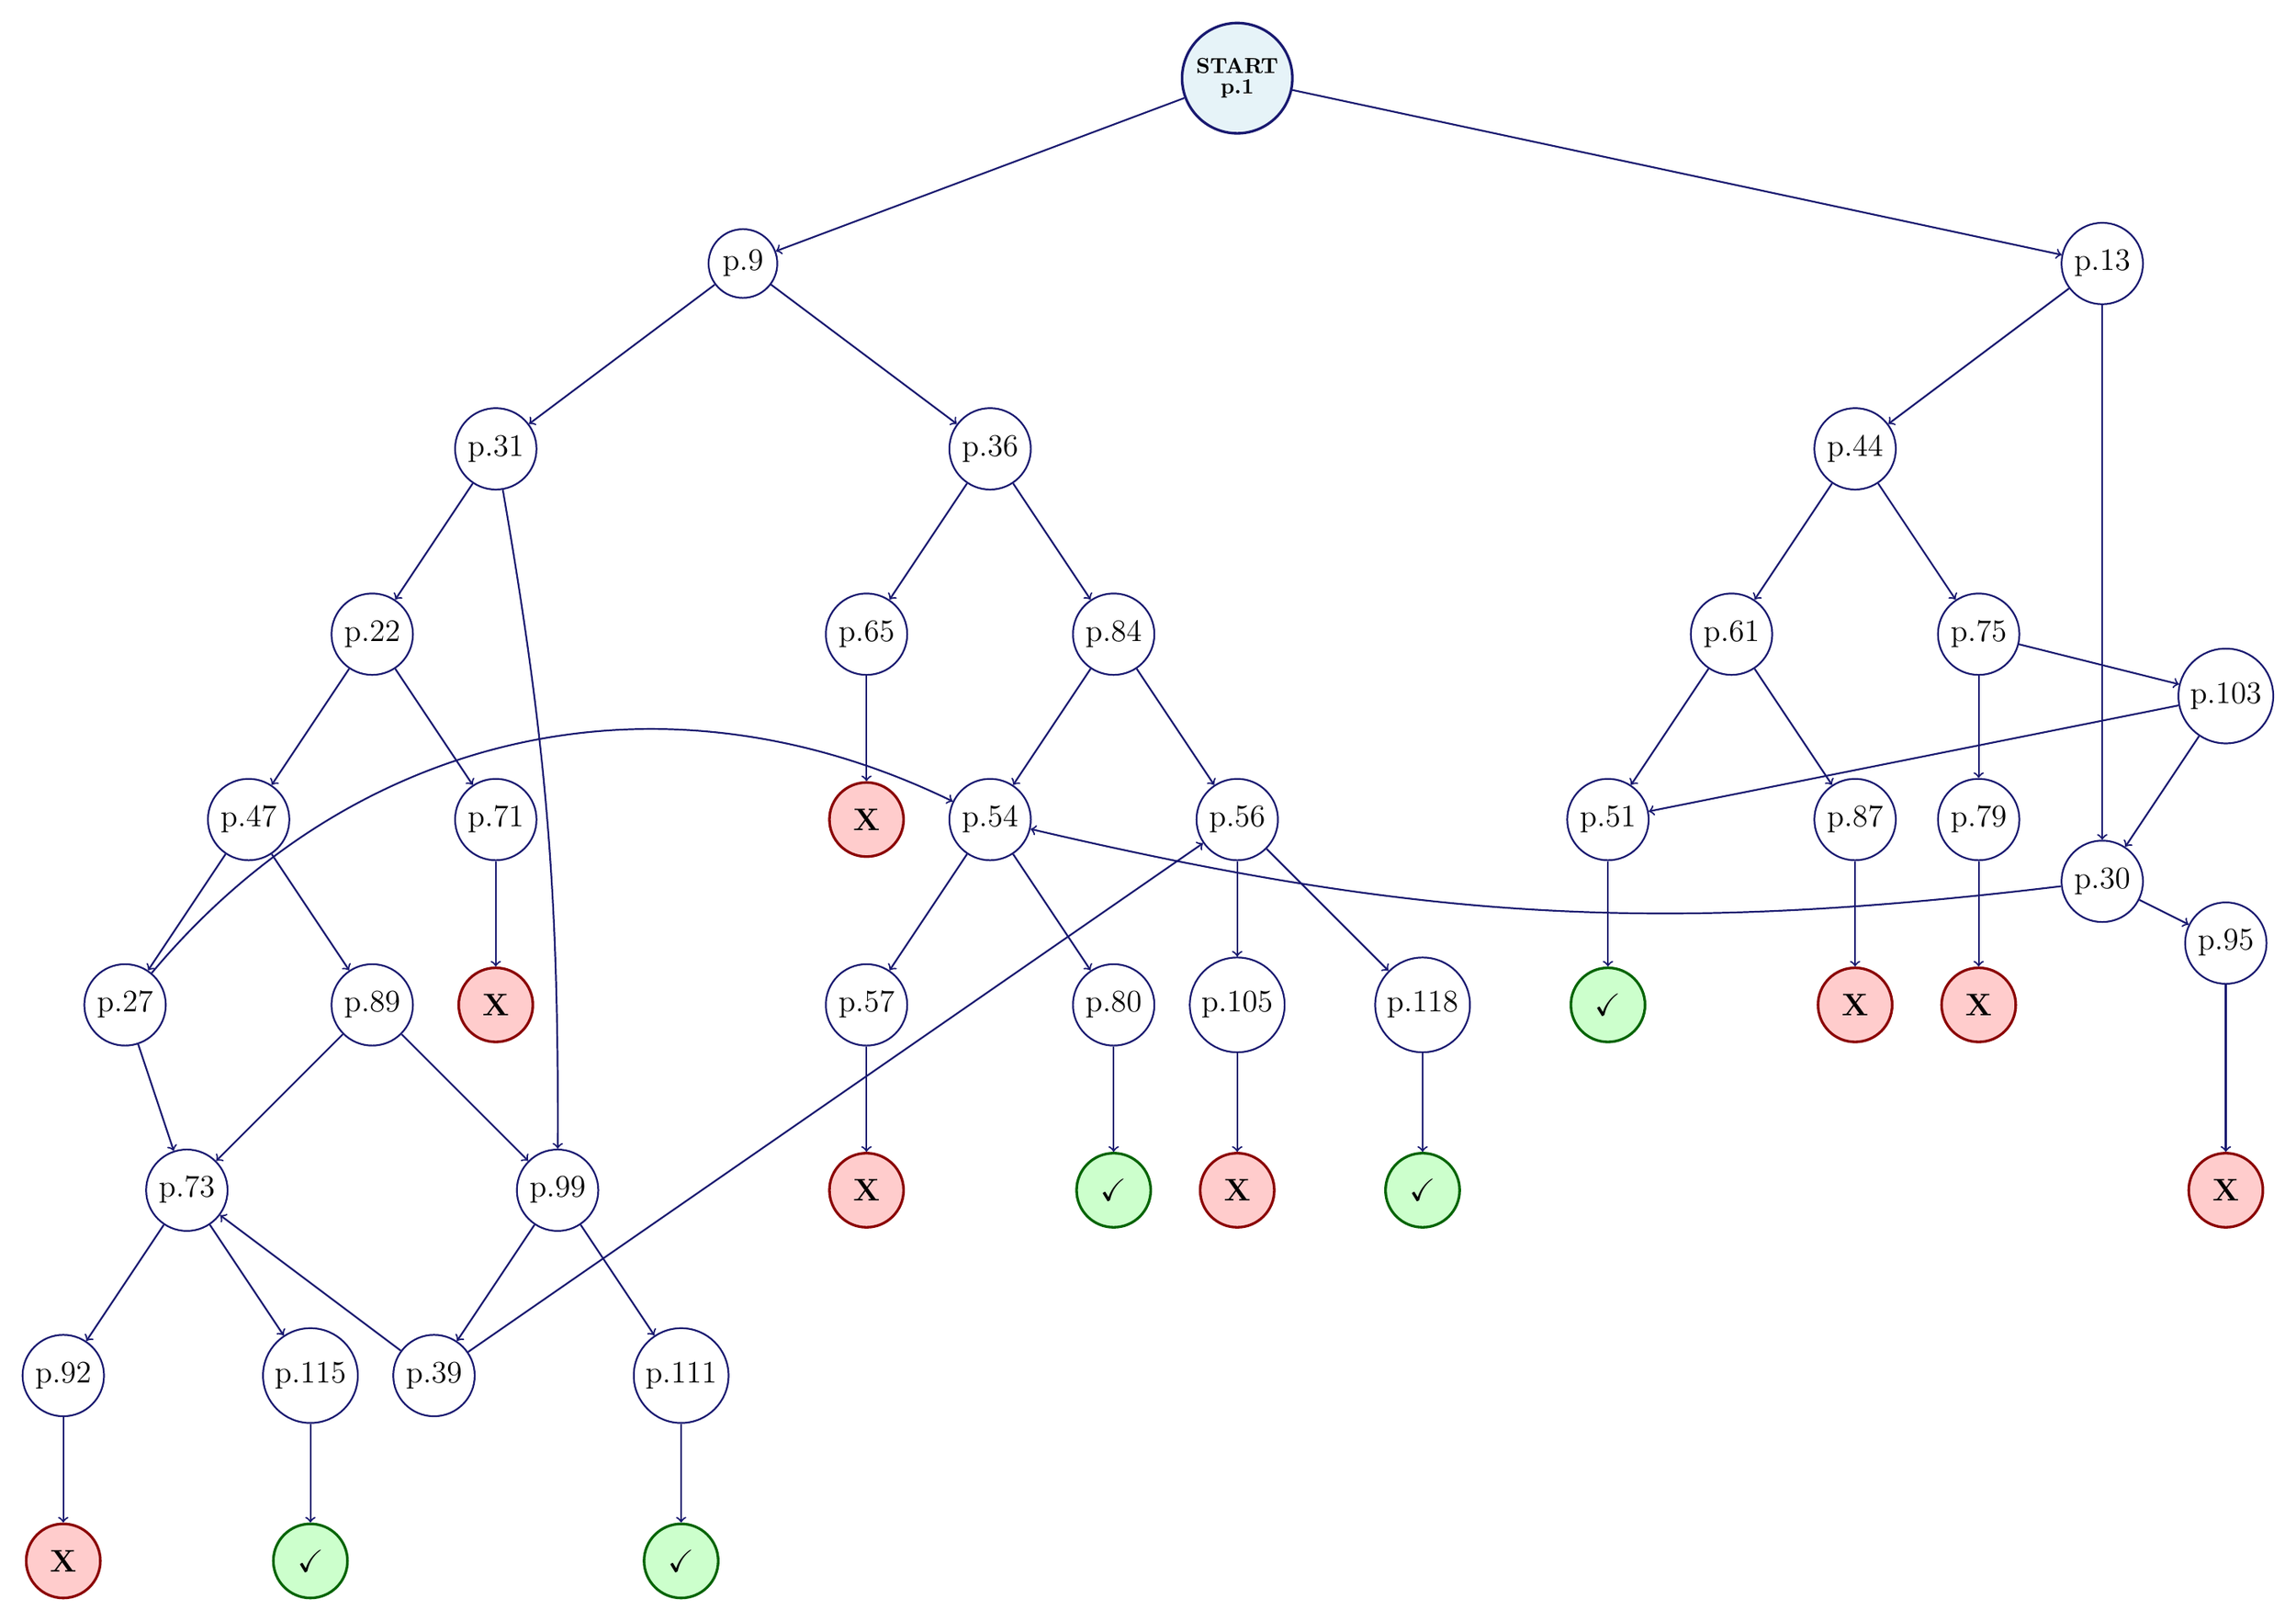
\begin{tikzpicture}[
    % Node styles
    start/.style={circle, draw=darkblue, fill=lightblue!30, minimum size=16mm, very thick, font=\bfseries},
    page/.style={circle, draw=darkblue, minimum size=10mm, thick, font=\Large},
    success/.style={circle, draw=darkgreen, fill=green!20, minimum size=12mm, very thick, font=\bfseries},
    failure/.style={circle, draw=darkred, fill=red!20, minimum size=12mm, very thick, font=\bfseries},
    repeat/.style={diamond, draw=purple, fill=purple!20, minimum size=10mm, thick, font=\scriptsize},
    % Edge styles
    edge/.style={draw=darkblue, thick, ->}
]

% Level 0 - Start
\node[start] (start) at (0,0) {\shortstack{START\\p.1}};

% Level 1
\node[page] (p9) at (-8,-3) {p.9};
\node[page] (p13) at (14,-3) {p.13};

% Level 2 - Left branch from p.9
\node[page] (p31) at (-12,-6) {p.31};
\node[page] (p36) at (-4,-6) {p.36};

% Level 2 - Right branch from p.13
\node[page] (p44) at (10,-6) {p.44};

% Level 3 - From p.31
\node[page] (p22) at (-14,-9) {p.22};

% Level 3 - From p.36
\node[page] (p65) at (-6,-9) {p.65};
\node[page] (p84) at (-2,-9) {p.84};

% Level 3 - From p.44
\node[page] (p61) at (8,-9) {p.61};
\node[page] (p75) at (12,-9) {p.75};

% Level 4 - From p.22
\node[page] (p47) at (-16,-12) {p.47};
\node[page] (p71) at (-12,-12) {p.71};

% Level 4 - From p.65
\node[failure] (x1) at (-6,-12) {\Large X};

% Level 4 - From p.84
\node[page] (p54) at (-4,-12) {p.54};
\node[page] (p56) at (0,-12) {p.56};

% Level 4 - From p.61
\node[page] (p51) at (6,-12) {p.51};
\node[page] (p87) at (10,-12) {p.87};

% Level 4 - From p.75
\node[page] (p79) at (12,-12) {p.79};
\node[page] (p103) at (16,-10) {p.103};

% Level 5 - From p.47
\node[page] (p27) at (-18,-15) {p.27};
\node[page] (p89) at (-14,-15) {p.89};

% Level 5 - From p.71
\node[failure] (x2) at (-12,-15) {\Large X};

% Level 5 - From p.54
\node[page] (p57) at (-6,-15) {p.57};
\node[page] (p80) at (-2,-15) {p.80};

% Level 5 - From p.56
\node[page] (p105) at (0,-15) {p.105};
\node[page] (p118) at (3,-15) {p.118};

% Level 5 - From p.51
\node[success] (win1) at (6,-15) {\Large $\checkmark$};

% Level 5 - From p.87
\node[failure] (x3) at (10,-15) {\Large X};

% Level 5 - From p.79
\node[failure] (x4) at (12,-15) {\Large X};

% Level 5 - From p.103
\node[page] (p30) at (14,-13) {p.30};

% Level 6 - From p.89
\node[page] (p73) at (-17,-18) {p.73};
\node[page] (p99) at (-11,-18) {p.99};

% Level 6 - From p.57
\node[failure] (x5) at (-6,-18) {\Large X};

% Level 6 - From p.80
\node[success] (win2) at (-2,-18) {\Large $\checkmark$};

% Level 6 - From p.105
\node[failure] (x6) at (0,-18) {\Large X};

% Level 6 - From p.118
\node[success] (win3) at (3,-18) {\Large $\checkmark$};

% Level 6 - From p.30b
\node[page] (p95) at (16,-14) {p.95};

% Level 7 - From p.73
\node[page] (p92) at (-19,-21) {p.92};
\node[page] (p115) at (-15,-21) {p.115};

% Level 7 - From p.99
\node[page] (p39) at (-13,-21) {p.39};
\node[page] (p111) at (-9,-21) {p.111};

% Level 7 - From p.95
\node[failure] (x7) at (16,-18) {\Large X};

% Level 8 - From p.92
\node[failure] (x8) at (-19,-24) {\Large X};

% Level 8 - From p.115
\node[success] (win4) at (-15,-24) {\Large $\checkmark$};

% Level 8 - From p.111
\node[success] (win5) at (-9,-24) {\Large $\checkmark$};

% Draw all edges
\draw[edge] (start) -- (p9);
\draw[edge] (start) -- (p13);

\draw[edge] (p9) -- (p31);
\draw[edge] (p9) -- (p36);

\draw[edge] (p13) -- (p30);
\draw[edge] (p13) -- (p44);

\draw[edge] (p31) -- (p22);
\draw[edge] (p31)  to[bend left=5] (p99);

\draw[edge] (p36) -- (p65);
\draw[edge] (p36) -- (p84);

\draw[edge] (p44) -- (p61);
\draw[edge] (p44) -- (p75);

\draw[edge] (p22) -- (p47);
\draw[edge] (p22) -- (p71);

\draw[edge] (p65) -- (x1);

\draw[edge] (p84) -- (p54);
\draw[edge] (p84) -- (p56);

\draw[edge] (p61) -- (p51);
\draw[edge] (p61) -- (p87);

\draw[edge] (p75) -- (p79);
\draw[edge] (p75) -- (p103);

\draw[edge] (p47) -- (p27);
\draw[edge] (p47) -- (p89);

\draw[edge] (p71) -- (x2);

\draw[edge] (p54) -- (p57);
\draw[edge] (p54) -- (p80);

\draw[edge] (p56) -- (p105);
\draw[edge] (p56) -- (p118);

\draw[edge] (p51) -- (win1);

\draw[edge] (p87) -- (x3);

\draw[edge] (p79) -- (x4);

\draw[edge] (p103) -- (p30);
\draw[edge] (p103) -- (p51);

\draw[edge] (p27) to[bend left=38] (p54);
\draw[edge] (p27) -- (p73);

\draw[edge] (p89) -- (p73);
\draw[edge] (p89) -- (p99);

\draw[edge] (p57) -- (x5);

\draw[edge] (p80) -- (win2);

\draw[edge] (p105) -- (x6);

\draw[edge] (p118) -- (win3);

\draw[edge] (p30) to[bend left=10] (p54);
\draw[edge] (p30) -- (p95);

\draw[edge] (p73) -- (p92);
\draw[edge] (p73) -- (p115);

\draw[edge] (p99) -- (p39);
\draw[edge] (p99) -- (p111);

\draw[edge] (p95) -- (x7);

\draw[edge] (p92) -- (x8);

\draw[edge] (p115) -- (win4);

\draw[edge] (p39) -- (p56);
\draw[edge] (p39) -- (p73);

\draw[edge] (p111) -- (win5);

\end{tikzpicture}
}

\end{landscape}
\end{document}